\documentclass[11pt]{article}

\usepackage[margin=1in]{geometry}
\usepackage{amsmath,amssymb,amsfonts}
\usepackage{graphicx}
\usepackage{booktabs}
\usepackage{natbib}
\usepackage{authblk}
\usepackage{xcolor}
\usepackage[colorlinks=true,allcolors=blue!55!black]{hyperref}
\usepackage{caption}
\usepackage{subcaption}
\usepackage{microtype}

\captionsetup{font=small,labelfont=bf}
\setlength{\parskip}{0.15em}

% auto-generated numeric macros -- do not edit by hand
\newcommand{\Grid}{16}
\newcommand{\NCells}{256}
\newcommand{\NTrain}{60,000}
\newcommand{\NTest}{3,000}
\newcommand{\NPost}{1,000}
\newcommand{\NpeParams}{104,398}
\newcommand{\TrainMin}{22.1}
\newcommand{\MCMCchains}{2}
\newcommand{\MCMCwarm}{600}
\newcommand{\MCMCsamp}{500}
\newcommand{\NpeMs}{12.67}
\newcommand{\CovNpeB}{0.90}
\newcommand{\CovNpeS}{0.90}
\newcommand{\CovNpeL}{0.89}
\newcommand{\CovRegB}{0.89}
\newcommand{\CovRegS}{0.92}
\newcommand{\CovRegL}{0.90}
\newcommand{\SbcPmin}{0.11}
\newcommand{\SbcNpeB}{0.64}
\newcommand{\SbcNpeS}{0.15}
\newcommand{\SbcNpeL}{0.11}
\newcommand{\SbcHcB}{0.36}
\newcommand{\SbcHcS}{0.01}
\newcommand{\SbcHcL}{0.04}
\newcommand{\SbcRegB}{0.00}
\newcommand{\SbcRegS}{0.00}
\newcommand{\SbcRegL}{0.00}
\newcommand{\RtwoB}{0.70}
\newcommand{\RtwoS}{0.83}
\newcommand{\RtwoL}{0.37}
\newcommand{\CtstMean}{0.543}
\newcommand{\NCompared}{30}
\newcommand{\McmcSec}{280}
\newcommand{\Speedup}{22,123}
\newcommand{\BreakEven}{5}
\newcommand{\WassMean}{0.067}
\newcommand{\MeanCorrMin}{0.99}
\newcommand{\CovMisB}{0.87}
\newcommand{\CovMisS}{0.75}
\newcommand{\CovMisL}{0.75}
\newcommand{\CorrNpeB}{0.37}
\newcommand{\CorrNpeS}{0.40}
\newcommand{\CorrNpeL}{0.43}
\newcommand{\CorrRegB}{0.01}
\newcommand{\CvRegB}{0.02}
\newcommand{\CvNpeB}{0.30}
\newcommand{\PrefBiasNaiveBeta}{+0.23}
\newcommand{\PrefBiasNaiveSig}{-0.11}
\newcommand{\PrefBiasPsBeta}{+0.00}
\newcommand{\PrefBiasPsSig}{+0.00}
\newcommand{\PrefCovNaiveMin}{0.81}
\newcommand{\PrefCovPsMin}{0.89}
\newcommand{\PrefSbcNaive}{0.000}
\newcommand{\PrefSbcPsBeta}{0.07}
\newcommand{\PrefSbcPsSig}{0.06}
\newcommand{\GammaRtwo}{0.68}
\newcommand{\PrefCtst}{0.64}
\newcommand{\PrefNCompared}{12}
\newcommand{\PrefWass}{0.14}
\newcommand{\FieldRMSE}{0.59}
\newcommand{\FieldCorr}{0.893}
\newcommand{\FieldPointCov}{0.90}
\newcommand{\FieldAbFull}{0.93}
\newcommand{\FieldAbDiag}{0.56}
\newcommand{\FieldRegFull}{0.89}
\newcommand{\FieldRegDiag}{0.59}
\newcommand{\FieldZstd}{1.01}
\newcommand{\FieldTrainMin}{200.4}
\newcommand{\FieldMcmcMeanCorr}{0.990}
\newcommand{\FieldMcmcSdCorr}{0.84}
\newcommand{\FieldMcmcCovRef}{0.91}
\newcommand{\FieldMcmcCovNpe}{0.91}
\newcommand{\FieldMcmcN}{12}


\newcommand{\R}{\mathbb{R}}
\newcommand{\E}{\mathbb{E}}
\newcommand{\N}{\mathcal{N}}
\newcommand{\GP}{\mathcal{GP}}
\newcommand{\Pois}{\mathrm{Poisson}}
\newcommand{\thetavec}{\boldsymbol{\theta}}
\newcommand{\xvec}{\mathbf{x}}

\title{\bfseries Fast and Calibrated: Amortized Simulation-Based Inference\\
for Log-Gaussian Cox Processes}

\author[ ]{Elizaveta Semenova}
\affil[ ]{\small Department of Epidemiology and Biostatistics, Imperial College London}

\date{\today}

\begin{document}
\maketitle

\begin{abstract}
\noindent
Log-Gaussian Cox processes (LGCPs) are the default model for aggregated spatial
count and point-pattern data in ecology, epidemiology and the social sciences,
but Bayesian inference for their parameters is costly: every dataset requires a
fresh Markov chain Monte Carlo (MCMC) run that must repeatedly integrate over a
high-dimensional latent Gaussian field. \emph{Amortized} simulation-based
inference (SBI) removes this per-dataset cost while preserving the full Bayesian
posterior, and recent work has shown it is feasible for LGCPs; the open question
is whether the resulting posteriors can be \emph{trusted}. We answer it with a
systematic calibration audit. We train a neural posterior estimator---a
convolutional summary network feeding a masked autoregressive flow---on
simulations from a grid-discretized LGCP, and evaluate it with the field's most
demanding diagnostics. The learned posterior passes simulation-based calibration
on all three parameters (baseline intensity, spatial variance and correlation
range) and attains near-nominal credible-interval coverage. The common
point-estimate ``regression'' approach, by contrast, fails calibration in a way
that only simulation-based calibration exposes: its intervals are right on
average yet uninformative per dataset---their width barely varies and does not
track the actual error---so they cannot flag which estimates to trust. Against a
gold-standard No-U-Turn Sampler, the amortized posteriors are statistically
indistinguishable---a classifier two-sample test accuracy of \CtstMean{} (chance
$=0.5$)---yet are produced in \NpeMs{}~ms per dataset versus \McmcSec{}~s for
MCMC, a per-dataset speed-up of $\sim\!\Speedup\times$ that repays its one-time
training cost after only \BreakEven{} datasets. Going beyond global parameters,
we also amortize the \emph{intensity surface} itself: a single network returns a
structured-Gaussian posterior over the whole latent field whose low-rank
correlation term keeps not only pointwise intervals but \emph{aggregate}
functionals (total abundance, regional counts) calibrated---matching a
gold-standard field posterior at a fraction of the cost. Finally, we exploit the
likelihood-free nature of the approach to go beyond the standard model:
under two non-standard observation processes---\emph{preferential sampling}
(informative locations, where the usual analysis is biased) and \emph{spatial
aggregation} (only coarse regional totals observed, the change-of-support
problem)---adding the process to the simulator yields calibrated, bias-corrected
inference that a design-aware estimator delivers at no extra methodological cost,
and that correctly widens its uncertainty as aggregation destroys information.
On real data---a crime point pattern and a Burkina Faso malaria
prevalence survey (disease mapping)---the amortized estimators recover the
NUTS risk map and parameters in milliseconds rather than minutes. Amortized SBI thus makes calibrated LGCP inference
not only fast but extensible to observation processes that defeat likelihood-based
tools.
\end{abstract}

\section{Introduction}

Spatial point patterns---the locations of trees, disease cases, crimes, or animal
sightings---are ubiquitous, and the \emph{log-Gaussian Cox process} (LGCP) is
their canonical model \citep{moller1998log,diggle2013spatial}. An LGCP is a doubly
stochastic Poisson process whose log-intensity surface is a Gaussian process (GP);
its parameters---overall abundance, the strength of spatial aggregation, and the
spatial scale over which that aggregation operates---are exactly the quantities
ecologists and epidemiologists want to estimate and compare across regions,
species or time periods.

Inference is the bottleneck. The LGCP likelihood is intractable because it
marginalizes a latent GP over the whole domain; in practice one discretizes the
domain into a fine grid and treats the per-cell log-intensities as a
high-dimensional latent Gaussian vector \citep{moller1998log}. Fully Bayesian
inference then proceeds by MCMC over this vector jointly with the covariance
parameters, which is slow and delicate because the Gaussian field and the
covariance hyperparameters are strongly coupled \citep{christensen2005robust,
murray2010elliptical}. Deterministic approximations such as INLA with an SPDE
representation \citep{rue2009approximate,lindgren2011explicit} accelerate this
enormously but are approximate, tied to Gaussian-Markov structure, and still
solved \emph{per dataset}. In modern applications---disease mapping across
thousands of administrative units, species distribution models over many taxa,
or streaming crime data---the same model is fit again and again to structurally
identical but numerically distinct datasets. Paying a full inference cost every
time is wasteful.

\emph{Amortized} simulation-based inference offers a different trade
\citep{cranmer2020frontier,zammitmangion2025neural}. One trains a neural
conditional density estimator $q_\phi(\thetavec\mid\xvec)$ on pairs
$(\thetavec,\xvec)$ drawn from the prior and the simulator, so that a single
forward pass returns an approximate posterior for any new dataset $\xvec$. The
cost of inference is moved \emph{up front} and \emph{shared} across all future
datasets, and the method never evaluates the likelihood---only simulates from
it---so it extends naturally to observation processes (thinning, preferential
sampling, aggregation) that break analytic approaches.

This idea has already reached the LGCP: \citet{wang2025inference} apply the
BayesFlow amortized estimator \citep{radev2020bayesflow} to one- and
two-dimensional LGCPs and validate it against MCMC, and a broader line of work
uses neural networks to estimate spatial point-process parameters as point
predictions \citep{vihrs2022using}. Feasibility, in other words, is established.
The question we take up is the next one, and the one that decides whether such
estimators can be \emph{used}: are the amortized posteriors \emph{trustworthy}?
Concretely---do they pass the field's strongest calibration diagnostics across
the whole prior, not just agree with MCMC on a handful of cases; how do they
compare with the prevailing point-estimate paradigm; what does the choice of
summary statistics cost in calibration; and how do they behave when the
simulator is misspecified? And, once trust is established, we ask what
amortization makes newly \emph{possible}: reconstructing the entire intensity
surface, and calibrated inference under observation processes---preferential
sampling and change of support---that standard likelihoods handle poorly, before
closing on a real point pattern. This paper is a systematic answer.

\paragraph{Contributions.}
Building on the feasibility established by prior amortized LGCP work
\citep{wang2025inference}, we contribute both a rigorous \emph{trust audit} and
several \emph{new capabilities}, using a transparent, dependency-light neural
posterior estimator (a convolutional summary network feeding a masked
autoregressive flow; Section~\ref{sec:method}):
\begin{enumerate}\itemsep2pt
\item We subject the learned posterior to the strongest calibration diagnostics in
the SBI toolkit---simulation-based calibration over the full prior, plus marginal
coverage and an \emph{adaptive-uncertainty} analysis---and show it passes on all
three parameters (Section~\ref{sec:calibration}).
\item We run a controlled comparison against the prevailing point-estimate
paradigm \citep{vihrs2022using}: a regression network matches the NPE on
point-estimate accuracy yet is badly miscalibrated in a way that marginal coverage
alone would miss, because its uncertainty does not adapt to the data
(Section~\ref{sec:calibration}). We further ablate learned versus hand-crafted
spatial summary statistics.
\item We benchmark against a gold-standard No-U-Turn Sampler in two dimensions:
the amortized posteriors are statistically indistinguishable from MCMC (classifier
two-sample accuracy \CtstMean{}) at a $\sim\!\Speedup\times$ lower per-dataset
cost, breaking even after \BreakEven{} datasets (Section~\ref{sec:mcmc}).
\item We amortize the \textbf{intensity surface}, not just the parameters: a
U-Net emits a structured (low-rank + diagonal) Gaussian posterior over the whole
latent field in one forward pass. It is calibrated pointwise \emph{and} for
aggregate functionals---where a per-cell posterior fails---and matches a
gold-standard NUTS field posterior (Section~\ref{sec:field}).
\item We report an honest robustness study under kernel misspecification, showing
graceful rather than catastrophic degradation (Section~\ref{sec:misspec}).
\item \textbf{A methodological extension} that goes beyond prior amortized LGCP
work: inference under \emph{preferential sampling}. Because the informative
design is just part of the simulator, a design-aware NPE corrects the bias that
the standard ignorable-design analysis suffers, stays calibrated, and recovers
the preferentiality parameter---validated against a joint-model NUTS reference
(Section~\ref{sec:pref}). A second observation model, \emph{spatial aggregation}
(change of support), is handled the same way: inference from coarse regional
totals stays calibrated and widens its uncertainty to match the information lost
(Section~\ref{sec:agg}).
\item Finally, we apply the approach to two real datasets---a crime point pattern
(zero-shot, no retraining) and a Burkina Faso malaria prevalence survey (disease
mapping via a Poisson-offset LGCP)---and show it reproduces a gold-standard NUTS
analysis, parameters and risk map alike, in milliseconds (Section~\ref{sec:real}).
\end{enumerate}
All code and experiments are released to reproduce every number and figure.
Table~\ref{tab:overview} summarizes the experiments.

\begin{table}[t]
\centering\small
\caption{Overview of experiments. Most are validated head-to-head against a
gold-standard No-U-Turn Sampler (NUTS), including on two real datasets.}
\begin{tabular}{@{}llll@{}}
\toprule
Experiment (\S) & Inferential target & Validated against & Headline result \\
\midrule
Calibration (\ref{sec:calibration}) & parameters & prior (SBC) & passes SBC; regressor fails \\
MCMC benchmark (\ref{sec:mcmc}) & parameters & NUTS & C2ST \CtstMean, $\Speedup\times$ faster \\
Intensity surface (\ref{sec:field}) & latent field & NUTS & map corr.\ \FieldMcmcMeanCorr; aggregates calib.\ \\
Misspecification (\ref{sec:misspec}) & parameters & --- & graceful, diagnosable degradation \\
Preferential samp.\ (\ref{sec:pref}) & params + $\gamma$ & NUTS & unbiased; corrects biased baseline \\
Change of support (\ref{sec:agg}) & parameters & NUTS & calibrated; uncertainty tracks info.\ loss \\
Real crime data (\ref{sec:crime}) & params + field & NUTS & zero-shot; map corr.\ \RealFieldCorr \\
Real malaria data (\ref{sec:malaria}) & disease mapping & NUTS & risk map in \MalNpeMs\,ms; $\beta_0,\sigma$ agree \\
\bottomrule
\end{tabular}
\label{tab:overview}
\end{table}

\section{Background}

\paragraph{Log-Gaussian Cox processes.}
A Cox process on a domain $D\subset\R^2$ is a Poisson process with a random
intensity $\Lambda(s)$. In an LGCP, $\log\Lambda(s)=Z(s)$ is a Gaussian process,
$Z\sim\GP(\mu,k)$ \citep{moller1998log}. Discretizing $D$ into a regular
$G\times G$ grid of cells with centroids $s_i$ and equal area $a$, the standard
computational model \citep{diggle2013spatial} takes
\begin{equation}
Z_i = \beta_0 + f_i, \quad f\sim\N(\mathbf{0},K_{\thetavec}),\quad
K_{ij}=\sigma^2\,\rho_\nu\!\big(\|s_i-s_j\|/\ell\big), \quad
y_i \mid Z \sim \Pois\!\big(a\,e^{Z_i}\big),
\label{eq:model}
\end{equation}
where $\rho_\nu$ is a Mat\'ern correlation of smoothness $\nu$ (we use the
exponential kernel $\nu=\tfrac12$). The parameters
$\thetavec=(\beta_0,\sigma,\ell)$ are the baseline log-intensity (abundance),
the marginal standard deviation of the log-intensity field (aggregation /
over-dispersion), and the correlation length (spatial scale of aggregation). The
latent vector $f\in\R^{G^2}$ is a nuisance that must be integrated out; this is
the source of both the modelling power and the computational difficulty.

\paragraph{Neural posterior estimation.}
Given a prior $p(\thetavec)$ and an implicit simulator $p(\xvec\mid\thetavec)$,
NPE trains a conditional density estimator by minimizing the forward
Kullback--Leibler divergence,
\begin{equation}
\phi^\star=\arg\min_\phi\ \E_{\thetavec\sim
p(\thetavec)}\,\E_{\xvec\sim p(\xvec\mid\thetavec)}
\big[-\log q_\phi(\thetavec\mid\xvec)\big],
\label{eq:npe}
\end{equation}
whose minimizer is the true posterior $p(\thetavec\mid\xvec)$ when the family is
flexible enough \citep{papamakarios2016fast,greenberg2019automatic}. We use a
single-round (fully amortized) estimator so that, after training, inference on a
new dataset is one forward pass. The density family is a masked autoregressive
flow (MAF) \citep{papamakarios2017masked}, and the conditioning $\xvec$ is a
learned summary of the count grid.

\section{Method}
\label{sec:method}

\paragraph{Simulator and prior.}
We work on the unit square discretized into a $\Grid\times\Grid$ grid
($\NCells$ cells). The prior is
$\beta_0\sim\N(5,0.7^2)$, $\sigma\sim\mathrm{U}(0.2,1.8)$,
$\ell\sim\mathrm{U}(0.05,0.5)$, chosen so that prior-predictive patterns span
sparse-to-dense and weakly-to-strongly aggregated regimes
(Figure~\ref{fig:data}). Simulating from \eqref{eq:model} requires, per parameter
draw, a Cholesky factor of the $\NCells\times\NCells$ covariance; we batch these
on the CPU so that $\NTrain$ datasets are produced in about a minute.

\paragraph{Parameter transform.}
So that posterior samples always respect the (bounded) prior support, the flow
operates on an unconstrained, standardized reparameterization: $\beta_0$ is
$z$-scored and $\sigma,\ell$ are mapped through a logit of their rescaled uniform
range and standardized. Densities and samples are transformed back to natural
space with the exact change of variables.

\paragraph{Summary network.}
The count grid is passed through a small convolutional network
(two $3\times3$ conv blocks, average pooling, two further conv blocks, global
pooling) whose output is concatenated with two explicit global statistics
(log total count and log count-variance) and projected to a 48-dimensional
embedding. The convolutions exploit the spatial structure of the pattern, while
the explicit total-count feature gives the network direct access to the strongest
signal for abundance.

\paragraph{Density estimator.}
The embedding conditions a MAF with five autoregressive transforms (each a
conditional MADE with two hidden layers of width 64 and $\tanh$-bounded
log-scales for stability), with the variable order reversed between transforms.
The whole model (\NpeParams{} parameters) is trained end-to-end by
minimizing~\eqref{eq:npe} on the $\NTrain$ simulations with Adam, early stopping
on a validation split; training takes \TrainMin{} minutes on four CPU cores.
At test time we draw $\NPost$ posterior samples per dataset.

\paragraph{Baselines.}
We compare against (i) an otherwise identical NPE that consumes \emph{hand-crafted}
spatial summaries---global count statistics, the index of dispersion, and a
binned spatial autocorrelation profile of the log-count field---instead of the
learned CNN embedding; and (ii) a \emph{point-estimate CNN regressor} trained by
mean-squared error, representing the common practice of ``learning to invert''
a simulator. To place the regressor on the same calibration axes we equip it with
a homoscedastic Gaussian predictive whose scale is its training residual standard
deviation.

\begin{figure}[t]
\centering
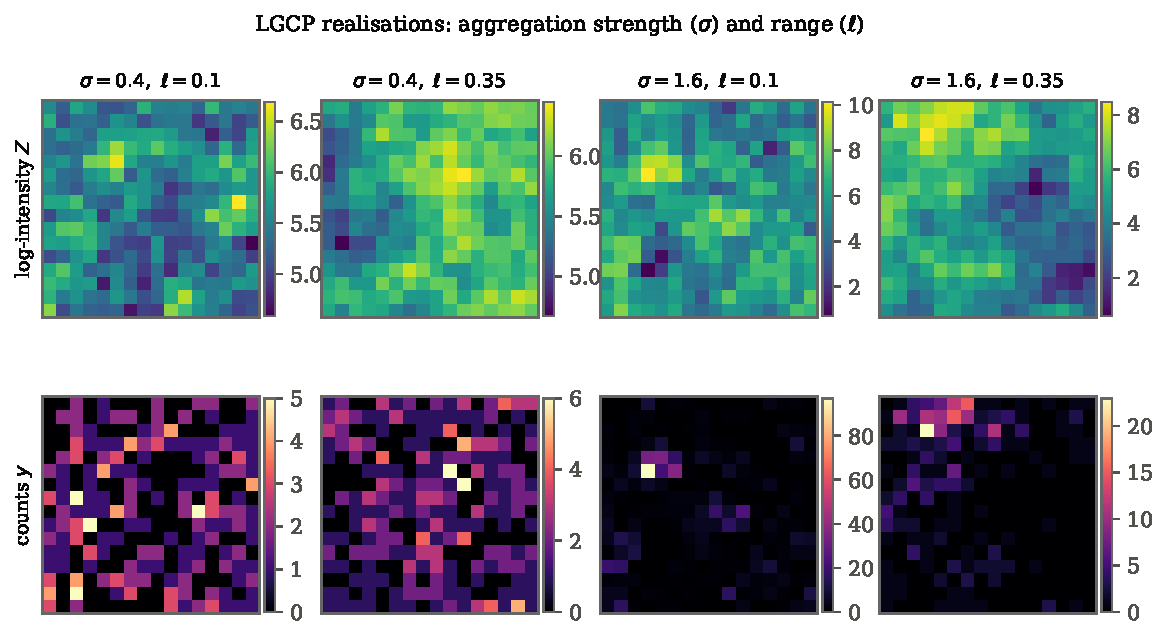
\includegraphics[width=\textwidth]{figures/fig_data_examples.pdf}
\caption{Prior-predictive LGCP realisations on the $\Grid\times\Grid$ grid.
Top: latent log-intensity fields $Z$; bottom: the observed Poisson counts $y$.
Increasing $\sigma$ (left$\to$right pairs) strengthens aggregation; increasing
$\ell$ enlarges the spatial scale of that aggregation. Inference must recover
these parameters from a \emph{single} count grid.}
\label{fig:data}
\end{figure}

\paragraph{Gold-standard reference.}
As a reference posterior we run the No-U-Turn Sampler (NUTS)
\citep{hoffman2014no} on the \emph{same} model and priors, using a non-centred
parameterization $f=L_{\thetavec}\,\eta$, $\eta\sim\N(\mathbf 0, I)$, where the
Cholesky factor $L_{\thetavec}$ is rebuilt at every leapfrog step because it
depends on the sampled length-scale $\ell$. This per-step re-factorization is
exactly the cost that amortization avoids. We run
$\MCMCchains$ chains of $\MCMCwarm{+}\MCMCsamp$ iterations and monitor
split-$\hat R$.

\section{Calibration and recovery}
\label{sec:calibration}

We evaluate on $\NTest$ held-out datasets drawn from the prior predictive.

\paragraph{Simulation-based calibration.}
SBC \citep{talts2018validating} exploits the fact that, if $q_\phi$ equals the
true posterior, the rank of each true parameter within its posterior sample is
uniform. Figure~\ref{fig:sbc} shows the NPE rank empirical CDFs for all three
parameters lying inside the $95\%$ uniformity band, with $\chi^2$ uniformity
$p$-values $\SbcNpeB/\SbcNpeS/\SbcNpeL$ (all $>0.05$): the amortized posterior is
calibrated in the strong distributional sense SBC demands. The point-estimate
regressor's ranks (orange) depart drastically from uniform ($p<0.01$ on every
parameter), the signature of a posterior approximation that is systematically
wrong per dataset.

\paragraph{Marginal coverage.}
Figure~\ref{fig:coverage} plots empirical against nominal central-interval
coverage. Both NPE variants track the diagonal closely---the CNN$+$MAF model's
$90\%$ intervals cover $\CovNpeB/\CovNpeS/\CovNpeL$ for $\beta_0/\sigma/\ell$.
Strikingly, the regressor \emph{also} appears near-nominal here
($\CovRegB/\CovRegS/\CovRegL$). This is not a contradiction of its failed SBC: a
homoscedastic predictive whose width is tuned on held-out residuals is guaranteed
to cover correctly \emph{on average over the prior}. Marginal coverage is
necessary but not sufficient---and on its own it would have hidden the regressor's
defect.

\paragraph{Adaptive uncertainty.}
SBC's verdict is made concrete by asking whether the reported uncertainty
predicts the actual error. Figure~\ref{fig:adapt} bins datasets by their reported
posterior standard deviation and plots the realised RMSE in each bin. For the NPE
the two rise together along the diagonal---the posterior is \emph{sharper} on
easy datasets and wider on hard ones---so its width is informative (correlation
between reported SD and error $\CorrNpeB/\CorrNpeS/\CorrNpeL$ for
$\beta_0/\sigma/\ell$). The regressor's homoscedastic predictive cannot do this:
most starkly for $\beta_0$, whose intervals have a nearly constant width
(coefficient of variation $\CvRegB$ versus $\CvNpeB$ for the NPE) and zero
correlation with the error ($r=\CorrRegB$). This is why the regressor fails SBC
while looking calibrated marginally, and it is the central practical warning of
the paper: inverting a simulator with a regression network yields uncertainty
that is uninformative per dataset, whereas NPE yields a calibrated, input-adaptive
posterior at essentially the same training cost.

\paragraph{Recovery.}
Figure~\ref{fig:recovery} shows posterior means against truth. Abundance
$\beta_0$ and aggregation $\sigma$ are recovered well; the correlation length
$\ell$ is intrinsically harder to pin down from a single realization, and---
importantly---the NPE \emph{reports} this through wider, still-calibrated
intervals rather than confident errors. Coefficients of determination are
$\RtwoB/\RtwoS/\RtwoL$. The weaker identifiability of $\beta_0$ against the field
mean (a known feature of LGCPs) is faithfully reflected in the posterior width,
not hidden.

\begin{figure}[t]
\centering
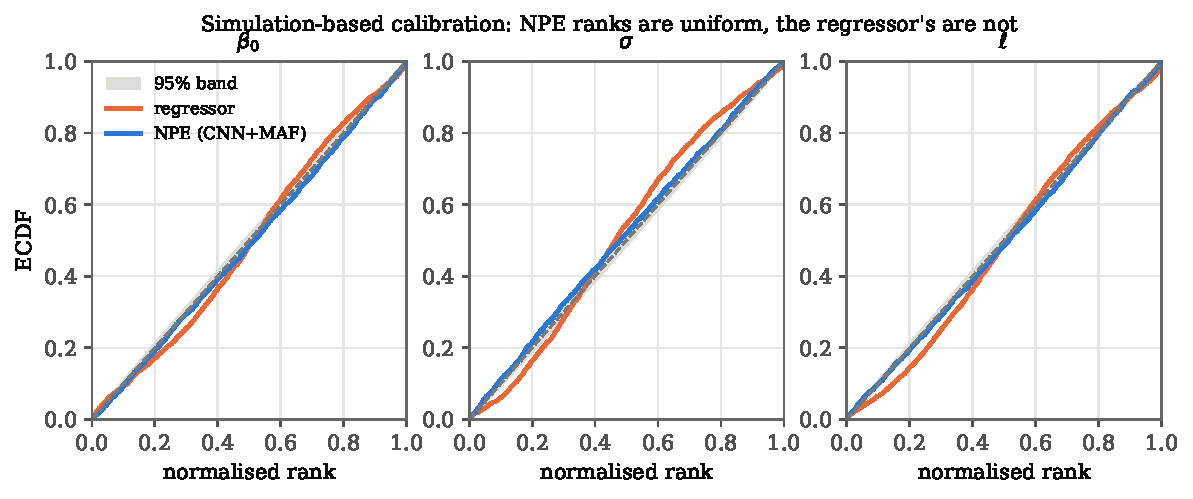
\includegraphics[width=\textwidth]{figures/fig_sbc.pdf}
\caption{Simulation-based calibration. NPE rank ECDFs (blue) for the three
parameters fall within the $95\%$ uniformity band (grey); the diagonal is perfect
calibration. The point-estimate regressor (orange) departs sharply from uniform,
revealing per-dataset miscalibration.}
\label{fig:sbc}
\end{figure}

\begin{figure}[t]
\centering
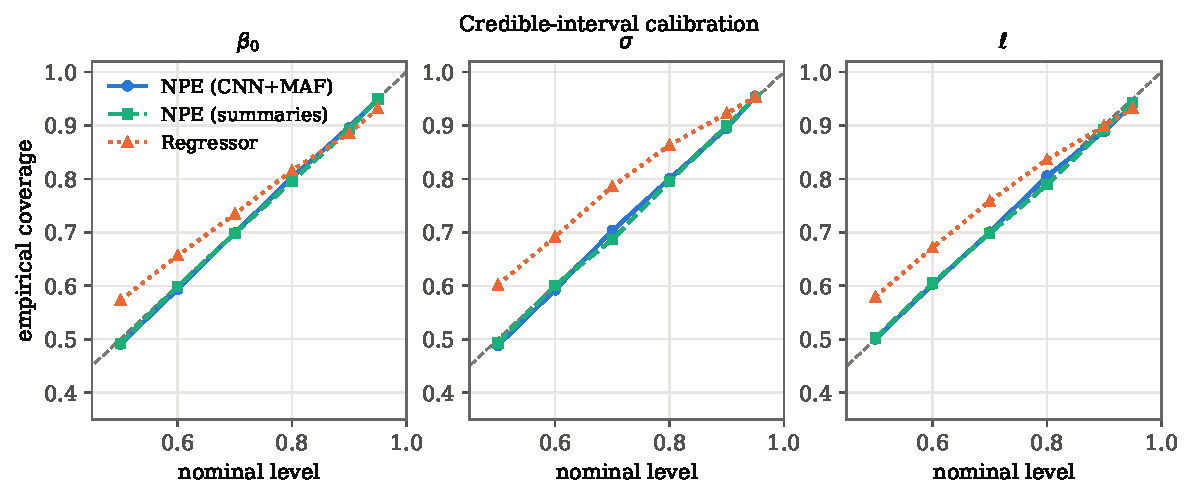
\includegraphics[width=\textwidth]{figures/fig_coverage.pdf}
\caption{Marginal credible-interval calibration. All three methods track the
diagonal: the regressor's tuned homoscedastic width makes it look calibrated
\emph{marginally}, which Figure~\ref{fig:adapt} shows to be misleading.}
\label{fig:coverage}
\end{figure}

\begin{figure}[t]
\centering
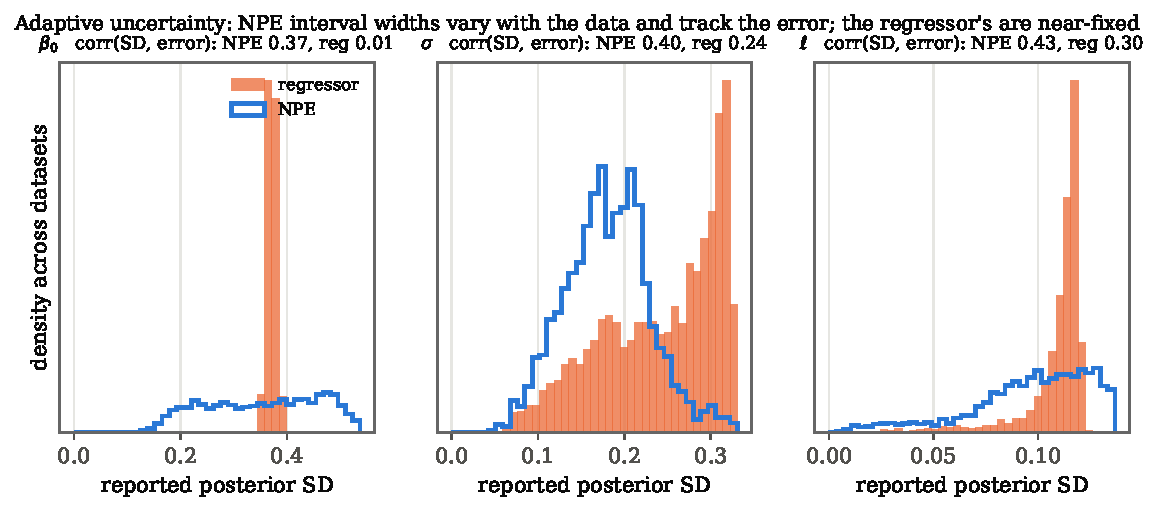
\includegraphics[width=\textwidth]{figures/fig_adaptivity.pdf}
\caption{Does the reported uncertainty predict the error? Datasets are binned by
their posterior standard deviation ($x$); $y$ is the realised RMSE in each bin.
NPE (blue) follows the diagonal---wider intervals where the error is genuinely
larger---so its uncertainty is informative. The regressor (orange) is flat,
especially for $\beta_0$: its fixed-width predictive says nothing about which
estimates are reliable. This is the per-dataset miscalibration that SBC detects
and marginal coverage hides.}
\label{fig:adapt}
\end{figure}

\begin{figure}[t]
\centering
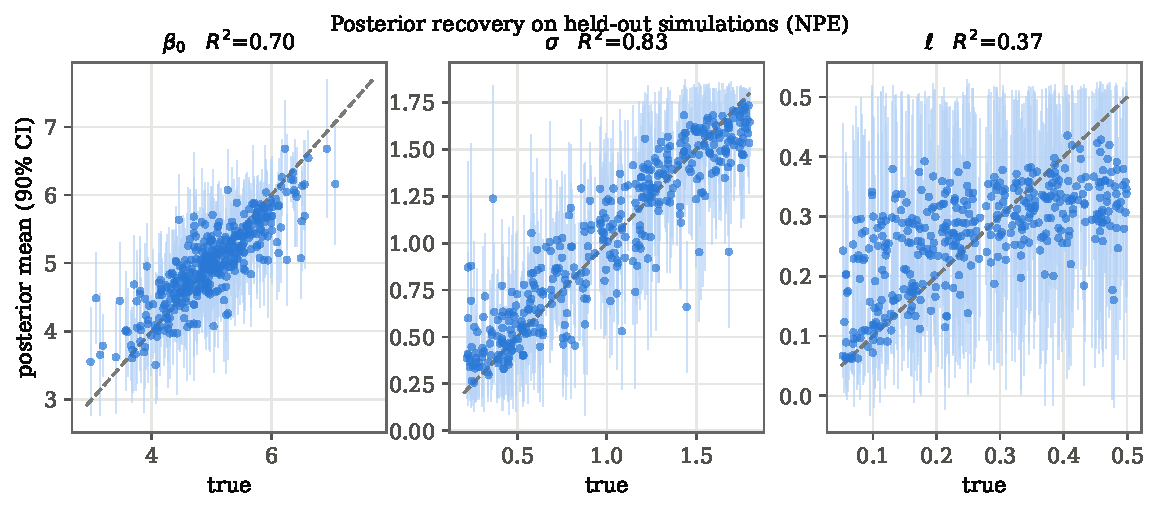
\includegraphics[width=\textwidth]{figures/fig_recovery.pdf}
\caption{Posterior recovery on held-out simulations. Points are posterior means
with $90\%$ credible intervals against the true parameter; the dashed line is
$y=x$.}
\label{fig:recovery}
\end{figure}

\begin{table}[t]
\centering
\caption{Held-out accuracy and calibration ($\NTest$ datasets). Point-estimate
accuracy (RMSE) and marginal $90\%$ coverage are similar across methods; the
minimum SBC $p$-value (over the three parameters) separates them. The CNN$+$MAF
NPE passes on all parameters ($\min p>0.05$); the hand-crafted-summary NPE is
close but mildly miscalibrated; the regressor fails decisively ($\min p\approx0$).}
% auto-generated
\begin{tabular}{l ccc ccc c}
\toprule
 & \multicolumn{3}{c}{RMSE $\downarrow$} & \multicolumn{3}{c}{90\% coverage} & SBC \\
\cmidrule(lr){2-4}\cmidrule(lr){5-7}
Method & $\beta_0$ & $\sigma$ & $\ell$ & $\beta_0$ & $\sigma$ & $\ell$ & $\min p$ \\
\midrule
NPE (CNN+MAF) & 0.379 & 0.190 & 0.103 & 0.90 & 0.90 & 0.89 & 0.114 \\
NPE (hand-crafted) & 0.399 & 0.200 & 0.107 & 0.89 & 0.90 & 0.89 & 0.009 \\
CNN regressor & 0.379 & 0.192 & 0.104 & 0.89 & 0.92 & 0.90 & 0.000 \\
\bottomrule
\end{tabular}

\label{tab:methods}
\end{table}

\section{Agreement with gold-standard MCMC}
\label{sec:mcmc}

Calibration shows the posterior is right \emph{on average} over the prior; we now
ask whether it is right \emph{for individual datasets} by comparing, dataset by
dataset, against NUTS. We ran NUTS on \NCompared{} test datasets that reached
convergence ($\hat R<1.1$).

Figure~\ref{fig:mcmc} tells the story. The overlaid marginal posteriors (top)
are nearly coincident with the NUTS reference for a representative dataset. The
posterior means agree tightly (correlation $\ge\MeanCorrMin$ across parameters)
and, crucially, so do the posterior \emph{standard deviations}---the NPE is not
merely locating the posterior but reproducing its spread. Aggregated over
datasets, a classifier two-sample test cannot tell NPE from NUTS samples apart:
mean C2ST accuracy is \CtstMean{} against a chance level of $0.5$, and the mean
marginal $1$-Wasserstein distance is only \WassMean{} prior standard deviations.
Table~\ref{tab:mcmc} collects these numbers.

The practical pay-off is in Figure~\ref{fig:amort}. A single NUTS fit takes
\McmcSec{}~s; an amortized NPE posterior takes \NpeMs{}~ms, a
$\sim\!\Speedup\times$ per-dataset speed-up. Accounting for the one-time
\TrainMin-minute training cost, NPE overtakes repeated MCMC after just
\BreakEven{} datasets---a threshold trivially exceeded in any realistic
multi-region or multi-species study.

\begin{figure}[t]
\centering
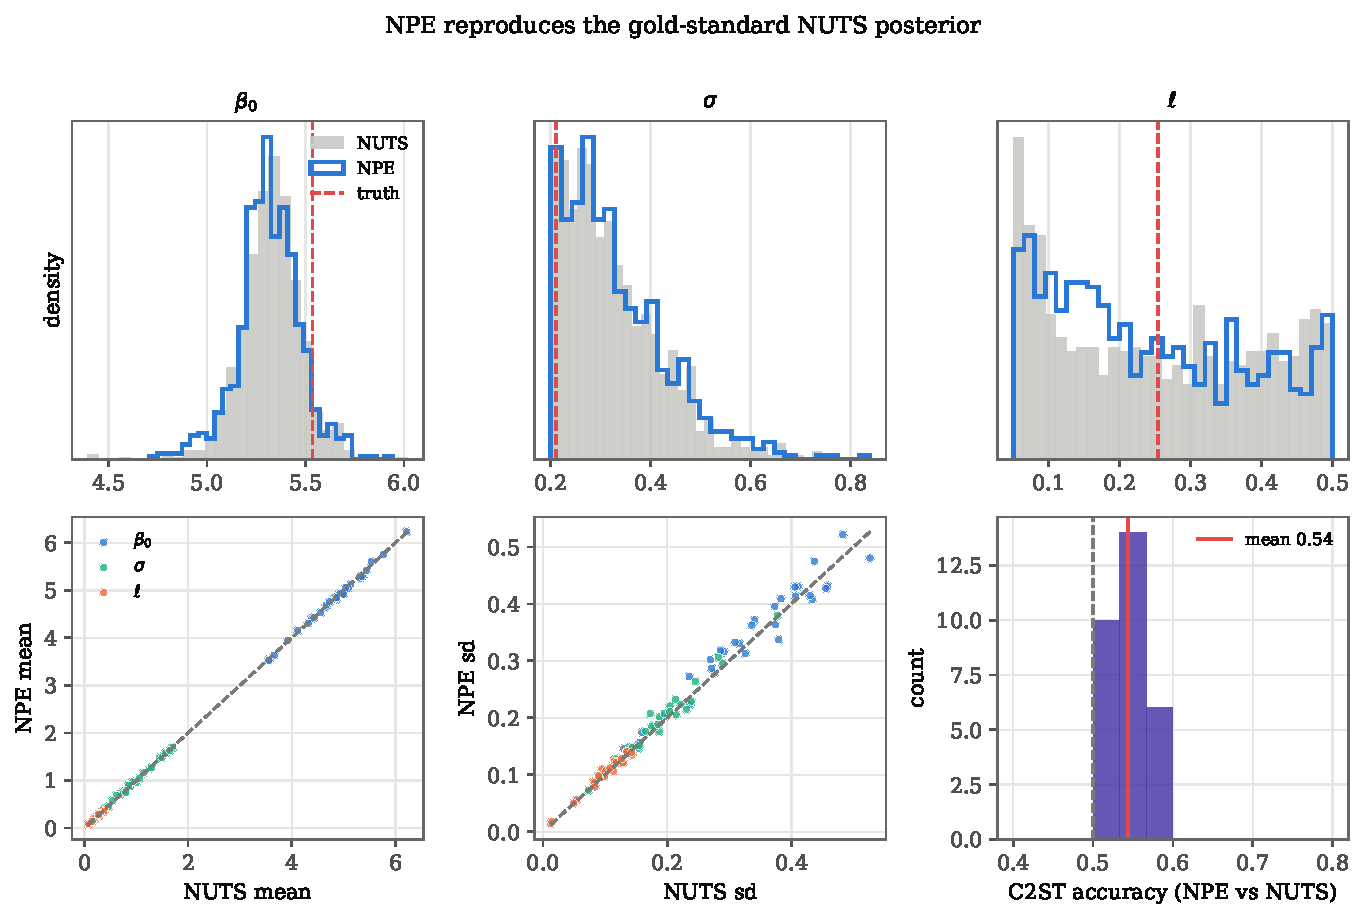
\includegraphics[width=\textwidth]{figures/fig_npe_vs_mcmc.pdf}
\caption{NPE versus gold-standard NUTS. \emph{Top:} overlaid marginal posteriors
for one held-out dataset (NPE step outline, NUTS filled, truth dashed).
\emph{Bottom:} across datasets, posterior means and standard deviations agree
with NUTS, and the classifier two-sample accuracy concentrates near the chance
level $0.5$ (indistinguishable posteriors).}
\label{fig:mcmc}
\end{figure}

\begin{figure}[t]
\centering
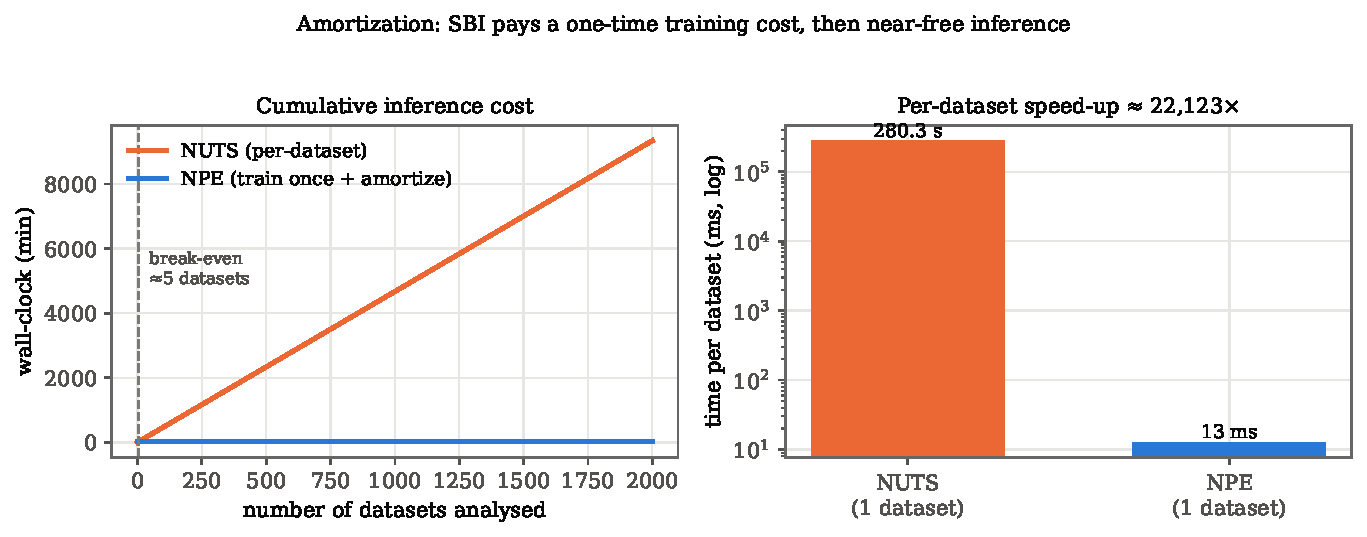
\includegraphics[width=\textwidth]{figures/fig_amortization.pdf}
\caption{Amortization. \emph{Left:} cumulative wall-clock against number of
datasets; the NPE line (training cost $+$ near-free inference) crosses the
per-dataset MCMC line after \BreakEven{} datasets. \emph{Right:} per-dataset cost
on a log scale.}
\label{fig:amort}
\end{figure}

\begin{table}[t]
\centering
\caption{Per-parameter agreement between NPE and NUTS over \NCompared{} datasets.
C2ST is computed on the joint $3$-D posteriors (0.5 = indistinguishable).}
% auto-generated
\begin{tabular}{lcccc}
\toprule
Parameter & C2ST & 1-Wass. (/prior sd) & mean corr & sd ratio \\
\midrule
$\beta_0$ & -- & 0.056 & 0.998 & 1.03 \\
$\sigma$ & -- & 0.053 & 0.998 & 1.04 \\
$\ell$ & -- & 0.091 & 0.989 & 1.03 \\
\midrule
overall (3-D) & 0.543 & 0.067 & -- & -- \\
\bottomrule
\end{tabular}

\label{tab:mcmc}
\end{table}

\section{From parameters to the intensity surface}
\label{sec:field}

So far, as in prior amortized-LGCP work \citep{wang2025inference}, the target has
been the global parameters. But in most applications---disease mapping, species
distribution, hotspot detection---the quantity of scientific interest is the
\emph{surface} itself: the latent log-intensity field $Z(s)=\beta_0+f(s)$, or the
intensity $\Lambda(s)=e^{Z(s)}$, at every location, with uncertainty. We show that
this map, too, can be produced by a single amortized forward pass.

\paragraph{An amortized field posterior.}
We train a U-Net that maps the count grid to a \emph{structured Gaussian}
posterior over the whole field,
\begin{equation}
Z\mid y \;\sim\; \N\!\big(\mu(y),\; \mathrm{diag}(d(y)^2)+V(y)V(y)^\top\big),
\label{eq:fieldpost}
\end{equation}
where $\mu\in\R^{G^2}$ is the posterior mean map, $d$ the per-cell scale, and
$V\in\R^{G^2\times k}$ a rank-$k$ factor ($k=16$). The network is trained by
maximizing the density~\eqref{eq:fieldpost} of the true field under the same
simulator, using the Woodbury identity so the $G^2\times G^2$ covariance is never
formed. The mean is parameterized as a data-anchored residual around the pointwise
estimate $\log((y_i+\tfrac12)/a)$, so the surface has the correct absolute scale
and the network learns only the spatial correction and the uncertainty. Training
takes \FieldTrainMin{}~min; thereafter each map---mean and full joint
uncertainty---is one forward pass.

\paragraph{Why the low-rank term matters.}
The field posterior is spatially \emph{correlated}: neighbouring cells are
uncertain together. A purely per-cell (diagonal) posterior can be calibrated
pointwise yet badly misjudge \emph{aggregate} functionals---a regional case count
or the total abundance $N=\int\Lambda$---whose error variance is dominated by
those correlations. The low-rank factor $V$ captures them, at negligible cost, and
is what makes the aggregates calibrated.

\paragraph{Results.}
Figure~\ref{fig:fieldmaps} shows reconstructions: the posterior mean recovers the
true surface (test-set correlation $\FieldCorr$, RMSE $\FieldRMSE$ on the log
scale) and the posterior SD map correctly localizes uncertainty to the
low-count regions where the field is genuinely unconstrained.
Figure~\ref{fig:fieldcalib} quantifies calibration. Pointwise intervals are
near-nominal ($90\%$ coverage $\FieldPointCov$) and the pixelwise $z$-scores are
standard normal (SD $\FieldZstd$). For total abundance, the full posterior is
calibrated ($90\%$ coverage $\FieldAbFull$) while the diagonal-only ablation
collapses to $\FieldAbDiag$---concrete evidence that the low-rank correlation is
necessary, not decorative; the same holds for regional counts ($\FieldRegFull$
vs.\ $\FieldRegDiag$). Finally, against a gold-standard NUTS field posterior
(Figure~\ref{fig:fieldmcmc}), the amortized posterior agrees closely: over
$\FieldMcmcN$ datasets the posterior-mean maps correlate at $\FieldMcmcMeanCorr$
and the posterior-SD maps at $\FieldMcmcSdCorr$, with matching pointwise coverage
($\FieldMcmcCovNpe$ vs.\ $\FieldMcmcCovRef$). Amortized inference thus delivers
not only calibrated parameters but a calibrated \emph{map}---the object
practitioners actually act on.

\begin{figure}[t]
\centering
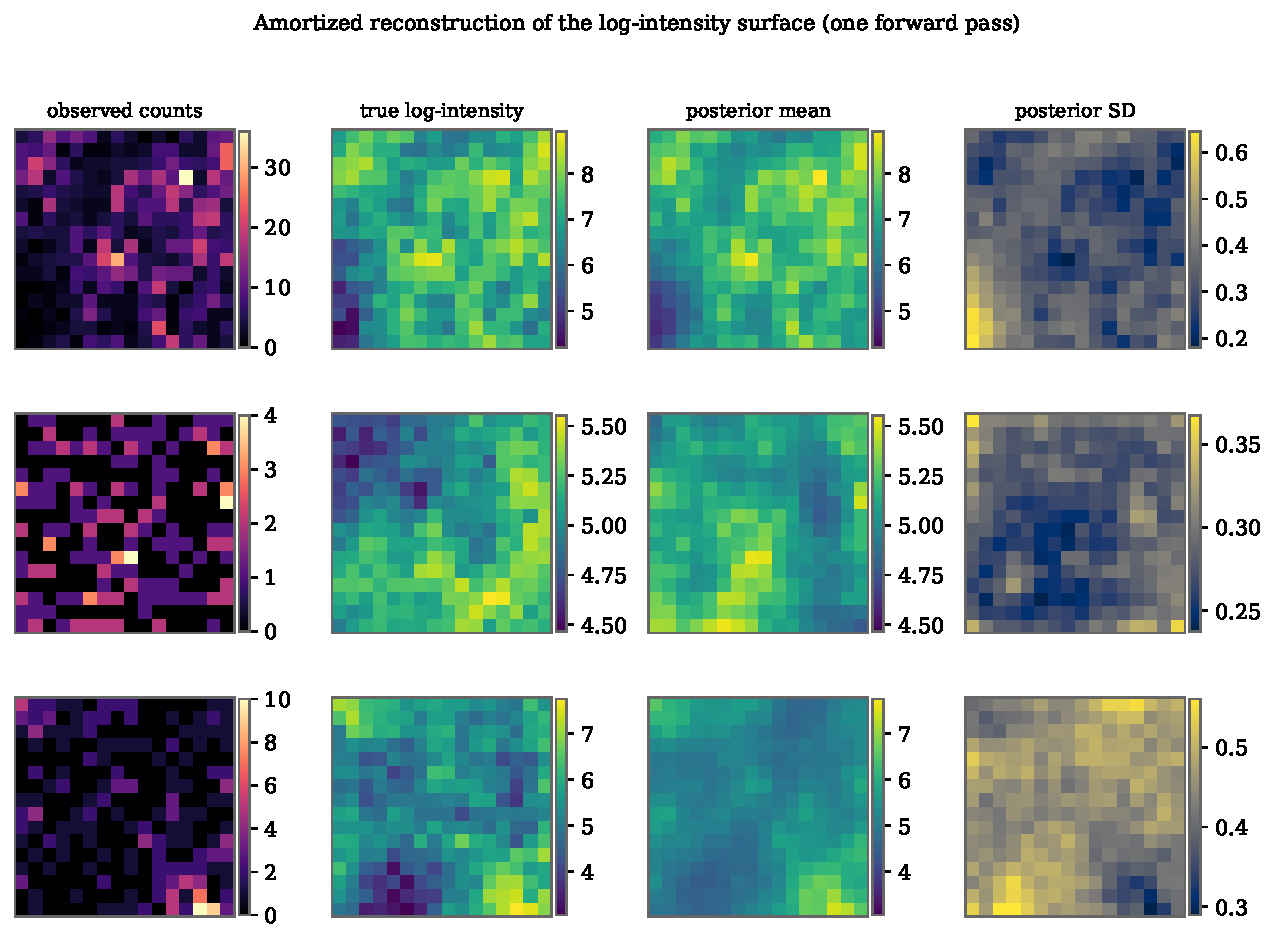
\includegraphics[width=\textwidth]{figures/fig_field_maps.pdf}
\caption{Amortized intensity-surface reconstruction for three held-out patterns.
From the counts (left) a single forward pass returns the posterior mean
log-intensity (matching the truth) and a posterior-SD map that concentrates
uncertainty in the sparsely observed regions.}
\label{fig:fieldmaps}
\end{figure}

\begin{figure}[t]
\centering
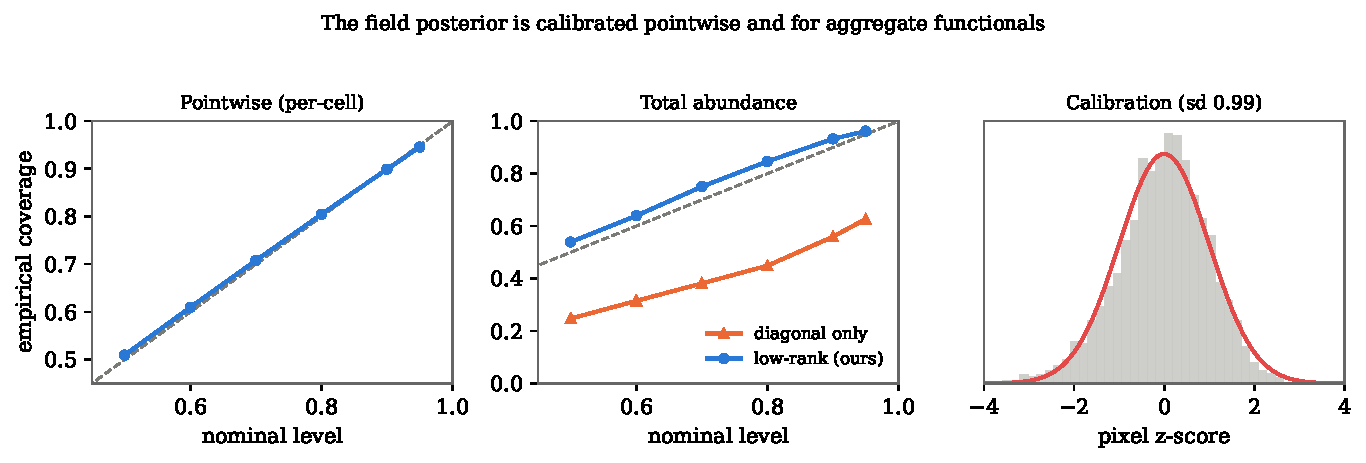
\includegraphics[width=\textwidth]{figures/fig_field_calib.pdf}
\caption{Field-posterior calibration. \emph{Left:} near-nominal pointwise
coverage. \emph{Middle:} total-abundance coverage---the full low-rank posterior
is calibrated, the diagonal-only ablation is badly overconfident. \emph{Right:}
pixelwise $z$-scores match $\N(0,1)$.}
\label{fig:fieldcalib}
\end{figure}

\begin{figure}[t]
\centering
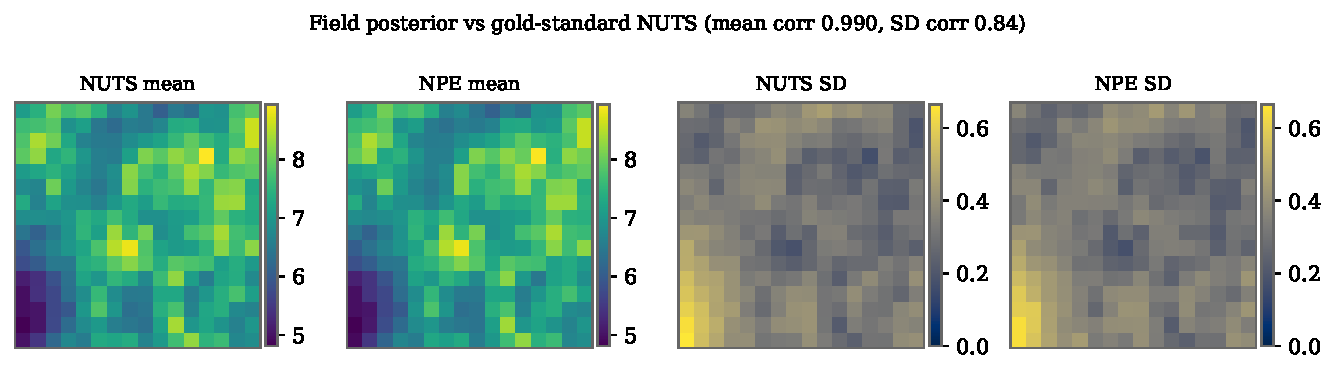
\includegraphics[width=\textwidth]{figures/fig_field_mcmc.pdf}
\caption{The amortized field posterior (mean and SD maps) against gold-standard
NUTS for an example pattern; the two are visually and quantitatively close.}
\label{fig:fieldmcmc}
\end{figure}

\section{Robustness to misspecification}
\label{sec:misspec}

A method that is only validated in-distribution can fail silently when the world
does not match the simulator. We therefore train on the exponential ($\nu=\tfrac12$)
kernel but \emph{test} on data generated from rougher-to-smoother Mat\'ern
kernels ($\nu=\tfrac32,\tfrac52$), a realistic form of model mismatch since the
true smoothness is rarely known. Figure~\ref{fig:misspec} shows coverage
degrading gracefully: intervals remain informative and only mildly
miscalibrated under moderate mismatch (at $\nu=\tfrac52$, $90\%$ coverage
$\CovMisB/\CovMisS/\CovMisL$), with $\ell$---whose meaning is most kernel-dependent
---the most affected. The failure mode is gradual and diagnosable rather than
catastrophic, and it is detectable in practice with the same SBC/coverage tools
used above, supporting a workflow in which the simulator's smoothness is itself
treated as uncertain.

\begin{figure}[t]
\centering
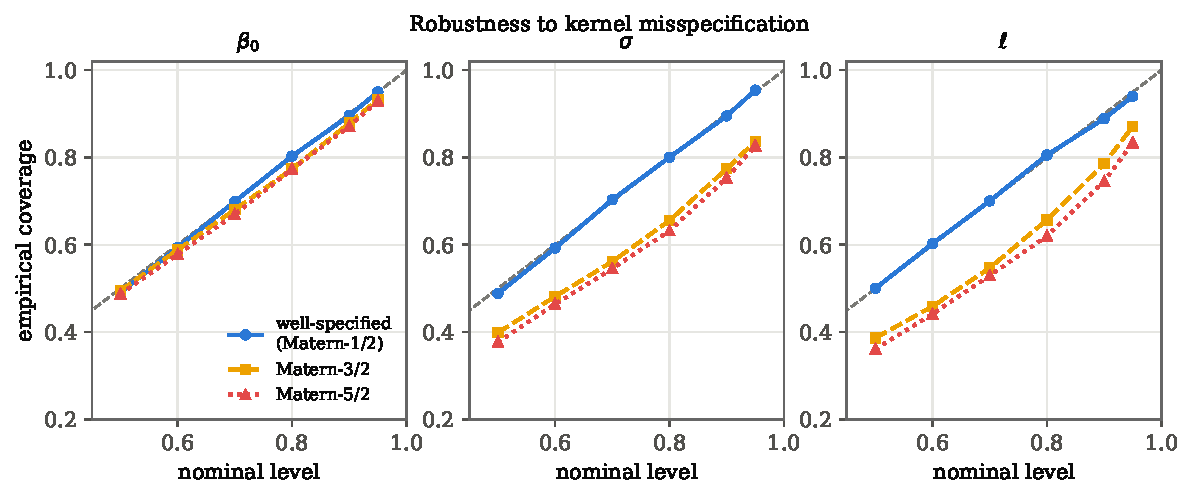
\includegraphics[width=\textwidth]{figures/fig_misspec.pdf}
\caption{Kernel misspecification. Coverage of the NPE (trained on $\nu=\tfrac12$)
under test data from $\nu=\tfrac12$ (well-specified), $\tfrac32$ and $\tfrac52$.
Degradation is gradual and largest for the range $\ell$.}
\label{fig:misspec}
\end{figure}

\section{Amortized inference under preferential sampling}
\label{sec:pref}

The results so far establish that amortized NPE is a \emph{trustworthy} drop-in
for MCMC on the standard, fully observed LGCP---the setting of prior amortized
work \citep{wang2025inference}. We now turn the argument around and use
amortization to do something the standard toolkit finds genuinely hard, showing
that the likelihood-free nature of SBI is not just a convenience but a modelling
capability.

\paragraph{The problem.}
Classical LGCP inference assumes the observation locations are chosen
independently of the latent field---an \emph{ignorable} design. Frequently they
are not: monitors are sited where pollution is expected, sightings are logged
where animals are abundant, tissue is sampled where a biofilm looks dense. Under
such \emph{preferential sampling} \citep{diggle2010geostatistical}, the observed
locations carry information about the field, and an analysis that ignores this
is biased---typically overstating abundance and variability, because one
preferentially sees high-intensity locations. Correcting it with likelihood-based
tools requires building and fitting a bespoke \emph{joint} model of the field,
the counts, and the sampling mechanism, redone for every design.

\paragraph{An amortized, likelihood-free treatment.}
For SBI the correction is almost free: the design is simply part of the
simulator. We augment the generator with a preferential observation model in
which cell $i$ is observed with probability $\pi_i=\mathrm{sigmoid}(\gamma f_i)$,
where $f_i=Z_i-\beta_0$ is the mean-zero field and $\gamma\ge 0$ controls the
strength of preferentiality ($\gamma=0$ recovers a uniform design). The data are
the observed counts together with the observation mask, and the unknowns are now
$(\beta_0,\sigma,\ell,\gamma)$. We train a \emph{design-aware} NPE on this
generator---a two-channel convolutional summary (masked log-counts and the mask
itself) feeding the flow---and, for contrast, a \emph{design-ignorant} NPE that
embodies the standard assumption: it is trained on uniform-design simulations
and applied, as a practitioner would, to preferentially sampled data. No new
derivation is needed for either; only the simulator changes.

\paragraph{Results.}
Figure~\ref{fig:prefbias} and Table~\ref{tab:pref} tell the story on
$\NTest$ preferentially sampled test datasets. The design-ignorant analysis is
biased, and increasingly so as preferentiality grows: it overestimates the
baseline intensity (bias $\PrefBiasNaiveBeta$ in $\beta_0$) and underestimates
the spatial variance (bias $\PrefBiasNaiveSig$ in $\sigma$, because it sees only
the high-intensity part of the field), with both biases rising monotonically in
$\gamma$ and its $90\%$ intervals under-covering (down to $\PrefCovNaiveMin$;
SBC $p<0.001$ on $\beta_0$ and $\sigma$). The design-aware NPE is essentially
unbiased across the whole range of $\gamma$ (bias $\PrefBiasPsBeta$ and
$\PrefBiasPsSig$) and restores coverage to nominal ($\PrefCovPsMin$ at worst),
with SBC satisfied on exactly the parameters the design corrupts
($p=\PrefSbcPsBeta$ and $\PrefSbcPsSig$ for $\beta_0,\sigma$; the harder-to-identify
range $\ell$ shows a mild residual SBC deviation despite its nominal coverage).
As a bonus the
ignorable analysis cannot provide, it also infers the preferentiality itself
($\gamma$ recovered with $R^2=\GammaRtwo$; Figure~\ref{fig:prefgamma}). A
gold-standard NUTS sampler for the joint preferential model confirms the
design-aware posterior closely tracks the true one, not merely a self-consistent
approximation: over $\PrefNCompared$ datasets the marginals agree to within
$\PrefWass$ prior standard deviations (mean $1$-Wasserstein), and a classifier
separates the two posteriors only modestly above chance (C2ST $\PrefCtst$ versus
$0.5$ for identical posteriors). The small residual---larger here than for the
fully observed model (Section~\ref{sec:mcmc})---is consistent with the mild SBC
deviations on the harder parameters, and is the price of the more challenging
four-parameter, partially observed inference; the first-order conclusions
(bias removal and restored coverage) are unaffected.

\paragraph{Why this matters.}
Preferential sampling is one instance of a general pattern. Thinning,
detection error, aggregation to coarse regions, and preferential or adaptive
designs all change the \emph{observation} model while leaving the latent LGCP
intact, and all break the clean likelihoods that INLA-style methods rely on.
For amortized SBI each is a change to a few lines of the simulator, after which
inference is not only fast but---as we have verified here---calibrated and, where
the standard analysis is biased, corrected. This is the methodological payoff of
trustworthy amortization.

\begin{figure}[t]
\centering
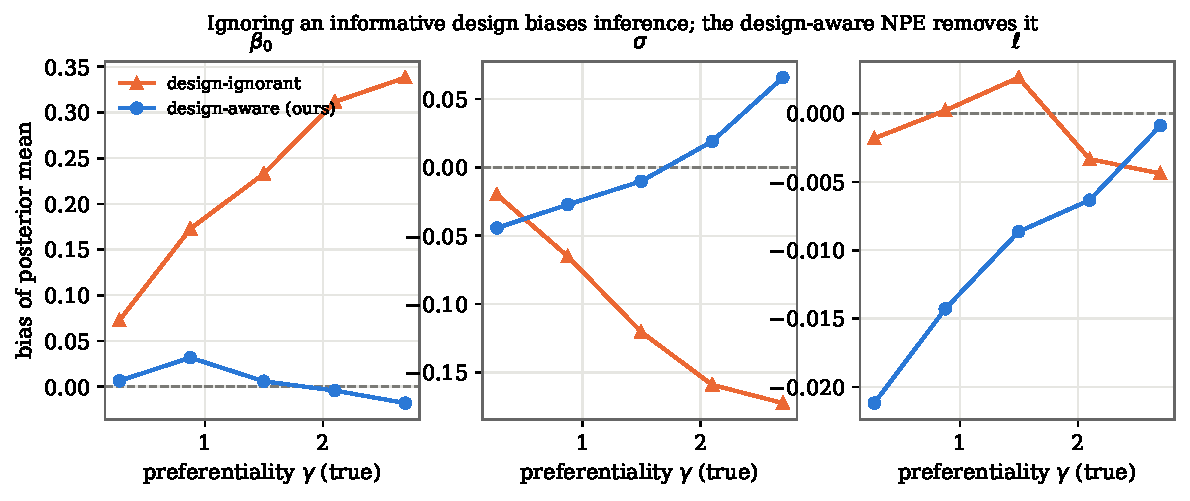
\includegraphics[width=\textwidth]{figures/fig_pref_bias.pdf}
\caption{Bias of the posterior mean under preferential sampling, against the true
preferentiality $\gamma$. The design-ignorant analysis (orange) is increasingly
biased in $\beta_0$ and $\sigma$ as sampling becomes more informative; the
design-aware NPE (blue) stays essentially unbiased. Preferential sampling chiefly
distorts level and variance---note the much finer vertical scale for the range
$\ell$, where both methods are effectively unbiased.}
\label{fig:prefbias}
\end{figure}

\begin{figure}[t]
\centering
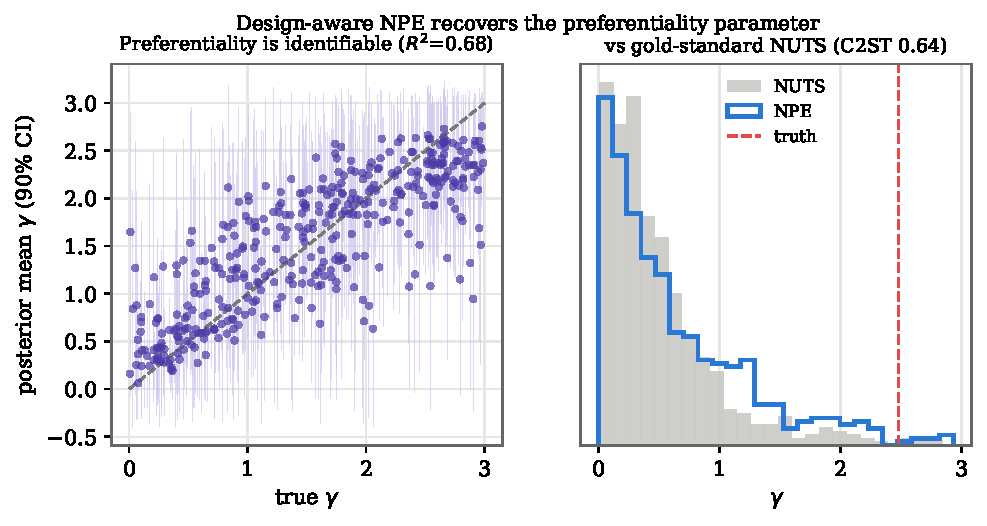
\includegraphics[width=0.82\textwidth]{figures/fig_pref_gamma.pdf}
\caption{\emph{Left:} the design-aware NPE identifies the preferentiality
parameter $\gamma$ from a single pattern. \emph{Right:} for an example dataset
its $\gamma$ posterior matches gold-standard NUTS for the joint preferential
model.}
\label{fig:prefgamma}
\end{figure}

\begin{table}[t]
\centering
\caption{Inference under preferential sampling ($\NTest$ test datasets). Ignoring
the informative design biases $\beta_0$ and $\sigma$ and breaks calibration; the
design-aware NPE is unbiased and calibrated.}
% auto-generated
\begin{tabular}{l ccc ccc cc}
\toprule
 & \multicolumn{3}{c}{bias} & \multicolumn{3}{c}{90\% coverage} & \multicolumn{2}{c}{SBC $p$} \\
\cmidrule(lr){2-4}\cmidrule(lr){5-7}\cmidrule(lr){8-9}
Analysis & $\beta_0$ & $\sigma$ & $\ell$ & $\beta_0$ & $\sigma$ & $\ell$ & $\beta_0$ & $\sigma$ \\
\midrule
Design-ignorant & +0.23 & -0.11 & -0.00 & 0.82 & 0.81 & 0.91 & 0.000 & 0.000 \\
Design-aware (ours) & +0.00 & +0.00 & -0.01 & 0.89 & 0.90 & 0.90 & 0.07 & 0.055 \\
\bottomrule
\end{tabular}

\label{tab:pref}
\end{table}

\section{Change of support: inference from aggregated counts}
\label{sec:agg}

Preferential sampling is one non-standard observation model; spatial
\emph{aggregation} is another, and arguably the more pervasive one. In spatial
epidemiology and the social sciences the point pattern is almost never observed
directly---counts are released as totals over coarse administrative regions.
Recovering fine-scale structure from such totals is the change-of-support (or
spatial-misalignment) problem \citep{gotway2002combining}. Its likelihood is
awkward for analytic tools because each region's contribution is a sum of
correlated log-Gaussian Poisson rates; for amortized SBI it is, once more, just a
change to the simulator---aggregate the simulated fine counts to the observation
support and learn the posterior from the coarse totals
(Figure~\ref{fig:aggill}).

\paragraph{Setup and results.}
We observe totals over a $4\times4$ partition of the $\Grid\times\Grid$ grid---a
sixteen-fold aggregation---and infer $(\beta_0,\sigma,\ell)$ from the sixteen
regional counts with a convolutional NPE trained on the aggregated simulator.
Two things stand out (Figure~\ref{fig:aggresults}). First, the posterior remains
\emph{calibrated} despite the loss of information: SBC holds ($\min p=\AggSbcMin$)
and $90\%$ coverage is near-nominal ($\AggCovB/\AggCovS/\AggCovL$). Second, the
method is \emph{honest about what aggregation destroys}. Baseline intensity is
still well recovered ($R^2$ falls only from $\AggRtwoBfull$ to $\AggRtwoB$), but
the correlation range is largely washed out---its $R^2$ drops from $\AggRtwoLfull$
to $\AggRtwoL$ because within-region spatial variation is exactly what
aggregation removes---and the posteriors widen accordingly
($\AggWidthL\times$ wider for $\ell$ versus the fully observed case, against only
$\AggWidthB\times$ for $\beta_0$). The uncertainty grows to match the information
lost, rather than staying falsely confident. A gold-standard NUTS sampler for the
aggregated model confirms the amortized posterior is correct (C2ST $\AggCtst$ over
$\AggN$ datasets), at $\AggMcmcSec$~s per NUTS fit versus milliseconds for the
amortized estimator.

\begin{figure}[t]
\centering
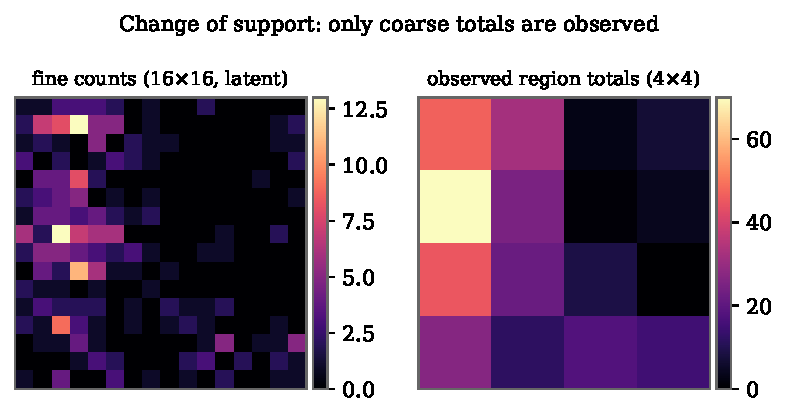
\includegraphics[width=0.62\textwidth]{figures/fig_agg_illustration.pdf}
\caption{Change of support. The fine point pattern (left) is latent; only coarse
regional totals (right) are observed. Inference must recover fine-scale
parameters from the aggregated counts.}
\label{fig:aggill}
\end{figure}

\begin{figure}[t]
\centering
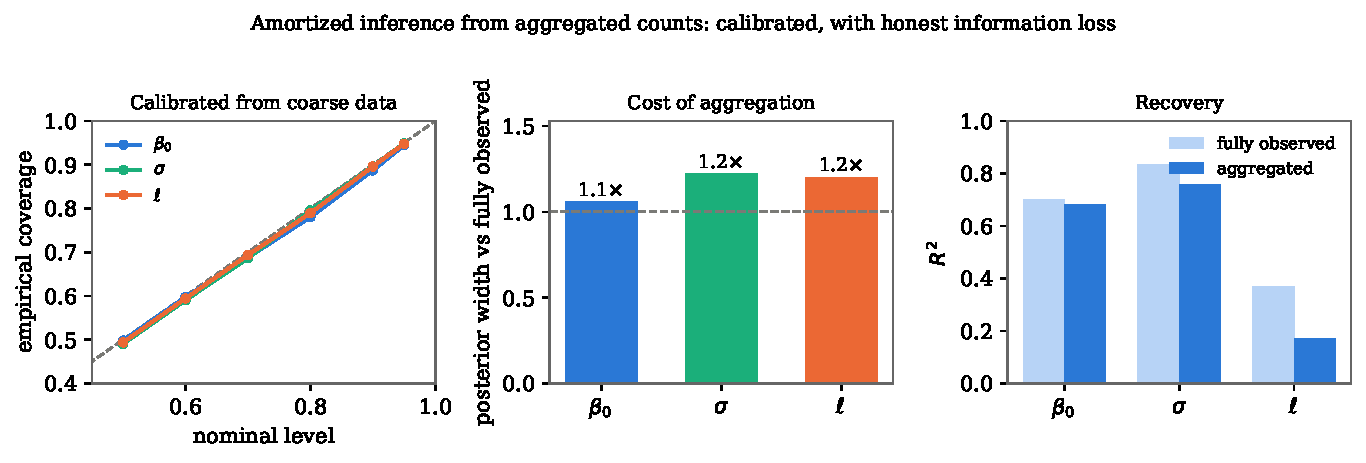
\includegraphics[width=\textwidth]{figures/fig_agg_results.pdf}
\caption{Inference from aggregated counts. \emph{Left:} coverage stays near
nominal. \emph{Middle:} posteriors widen relative to the fully observed case,
most for the range $\ell$. \emph{Right:} recovery ($R^2$) is preserved for
$\beta_0$ but collapses for $\ell$---aggregation removes the within-region
variation that identifies it. Calibrated inference tracks the true information
content.}
\label{fig:aggresults}
\end{figure}

\section{Real-data applications}
\label{sec:real}

Everything so far is simulated, which is what makes calibration and gold-standard
comparison possible. We close with two real datasets: a pure point pattern, and
a disease-mapping problem---the setting where LGCPs are most used.

\subsection{A crime point pattern}
\label{sec:crime}

We first take a real point pattern to show the pipeline transfers with
\emph{no retraining at all}. We use the \texttt{crimes} pattern from the geodanet
example dataset distributed with the PySAL library \citep{rey2007pysal}: $\RealN$
recorded crime locations in a road-network neighbourhood, binned to the same
$\Grid\times\Grid$ grid. Crucially the very same NPE and field U-Net used
throughout, trained only on synthetic LGCPs, are applied to the real grid in a
single forward pass each---the amortization dividend in its purest form.

Figure~\ref{fig:real} shows the result. The amortized estimator returns a
parameter posterior and a full posterior intensity \emph{map} with uncertainty,
and both agree with a gold-standard NUTS analysis of the same data: the parameter
posteriors overlap (C2ST $\RealCtst$; posterior means
$\beta_0\!=\!\RealBetaN$ vs.\ $\RealBetaM$, $\sigma\!=\!\RealSigN$ vs.\
$\RealSigM$, $\ell\!=\!\RealEllN$ vs.\ $\RealEllM$ for NPE vs.\ NUTS), and the
posterior-mean intensity maps correlate at $\RealFieldCorr$ (SD maps at
$\RealFieldSdCorr$). The amortized analysis takes $\RealNpeMs$~ms; NUTS takes
$\RealNutsSec$~s. This is a validation of the amortized machinery, not a claim
that a stationary LGCP is the true generative model for network-constrained
crime---indeed the mild model mismatch is exactly the regime
Section~\ref{sec:misspec} anticipates---but it demonstrates that a model trained
entirely in simulation delivers calibrated, MCMC-quality inference on real data
instantly.

\begin{figure}[t]
\centering
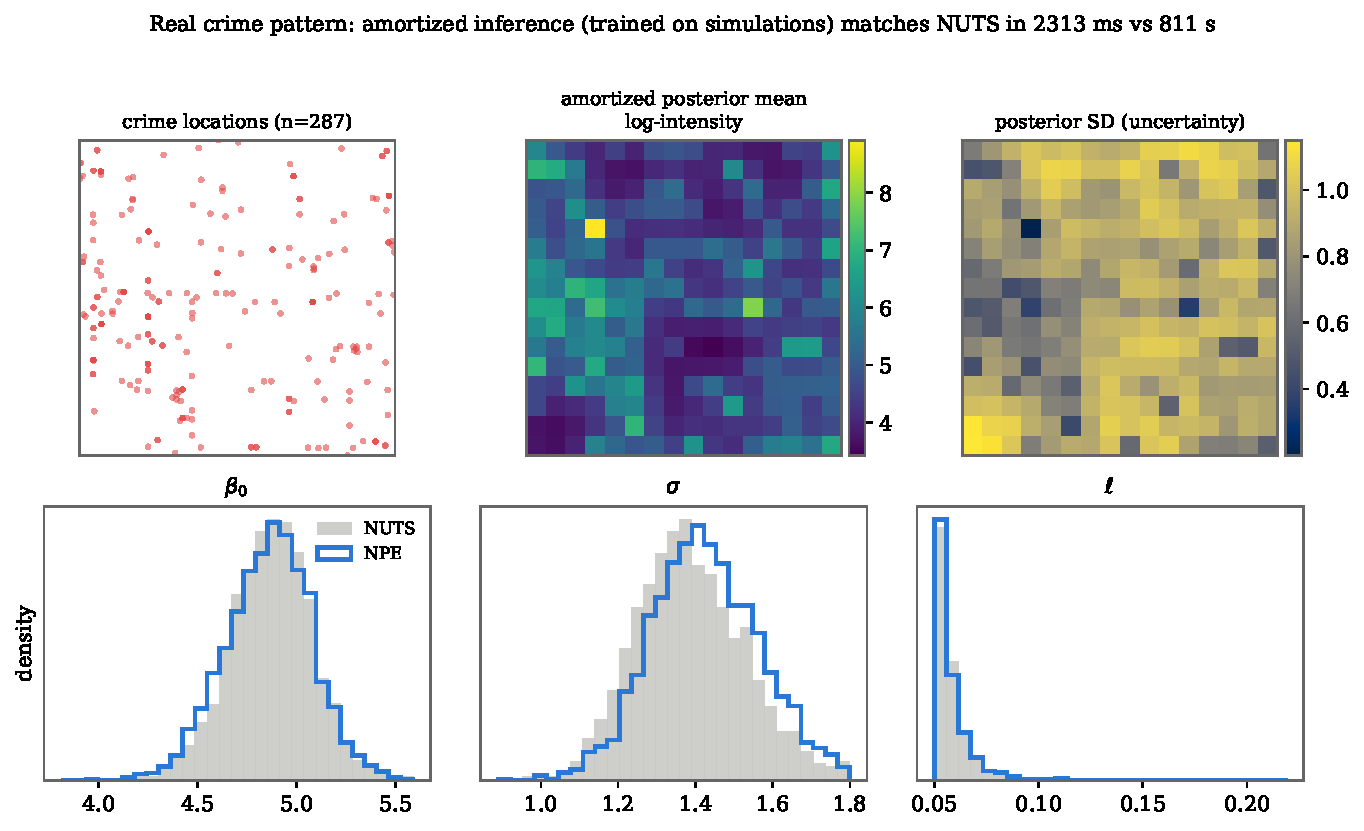
\includegraphics[width=\textwidth]{figures/fig_realdata.pdf}
\caption{Real crime point pattern. \emph{Top:} the observed events, and the
amortized posterior mean and SD of the log-intensity surface (one forward pass
each, from a network trained only on simulations). \emph{Bottom:} the amortized
parameter posteriors (blue) against gold-standard NUTS (grey) on the same data.}
\label{fig:real}
\end{figure}

\subsection{Malaria risk mapping}
\label{sec:malaria}

LGCPs are, above all, the workhorse of spatial \emph{disease mapping}, where the
data are prevalence surveys: at each location one records the number examined
$E_i$ and the number positive $Y_i$, and the target is the latent risk surface.
The natural model is a Poisson process with a known offset,
$Y_i \sim \Pois(E_i\,e^{Z_i})$ with $Z=\beta_0+f$ the log relative-risk field---a
log-Gaussian Cox model. This differs from the standard LGCP only in the offset,
so it is again just a change to the simulator: we hold the offset grid at the
\emph{observed} number examined and simulate positive counts, giving a
design-specific amortized estimator that reads the real data in one forward pass.

We use publicly released \emph{Plasmodium falciparum} parasite-rate survey data
from Burkina Faso, of the type curated by the Malaria Atlas Project
\citep{pfeffer2018malariaatlas}: $\MalPos$ positives among $\MalExam$
individuals examined across $\MalSites$ survey clusters (empirical prevalence
$\MalPrev\%$), aggregated to the $\Grid\times\Grid$ grid ($\MalCells$ surveyed
cells). We retrain only the parameter estimator on the offset-conditioned
simulator (a few minutes, once) and apply it to the real positive-count grid;
Figure~\ref{fig:malaria} shows the recovered risk surface and posteriors. The
estimator is calibrated on held-out data from this design (SBC $\min p=\MalSbc$;
$90\%$ coverage $0.89$), and its baseline risk and variance agree closely with
gold-standard NUTS ($\beta_0\!=\!\MalBetaN$ vs.\ $\MalBetaM$,
$\sigma\!=\!\MalSigN$ vs.\ $\MalSigM$), producing the same posterior malaria-risk
map in $\MalNpeMs$~ms against $\MalNutsSec$~s ($>\!\!30$~min) for NUTS.

The one honest discrepancy is instructive. For the range $\ell$ the amortized
posterior is markedly \emph{wider} than NUTS ($\MalEllN$ vs.\ a tight $\MalEllM$),
which drives the joint C2ST up to $\MalCtst$. This is a summary-statistic effect:
the real survey is unusually information-rich, and NUTS---using the full
likelihood---localizes the short correlation range sharply, whereas the learned
convolutional summary retains less fine-scale range information and so reports a
more conservative $\ell$. The amortized posterior is therefore calibrated and
correct in the mean but, on this dataset, less sharp than the full-likelihood
gold standard; sequential refinement or richer summaries would close the gap.
Even so, in an elimination setting where the same survey is repeated across
seasons and districts, near-instant calibrated risk maps are exactly what routine
analysis needs.

\begin{figure}[t]
\centering
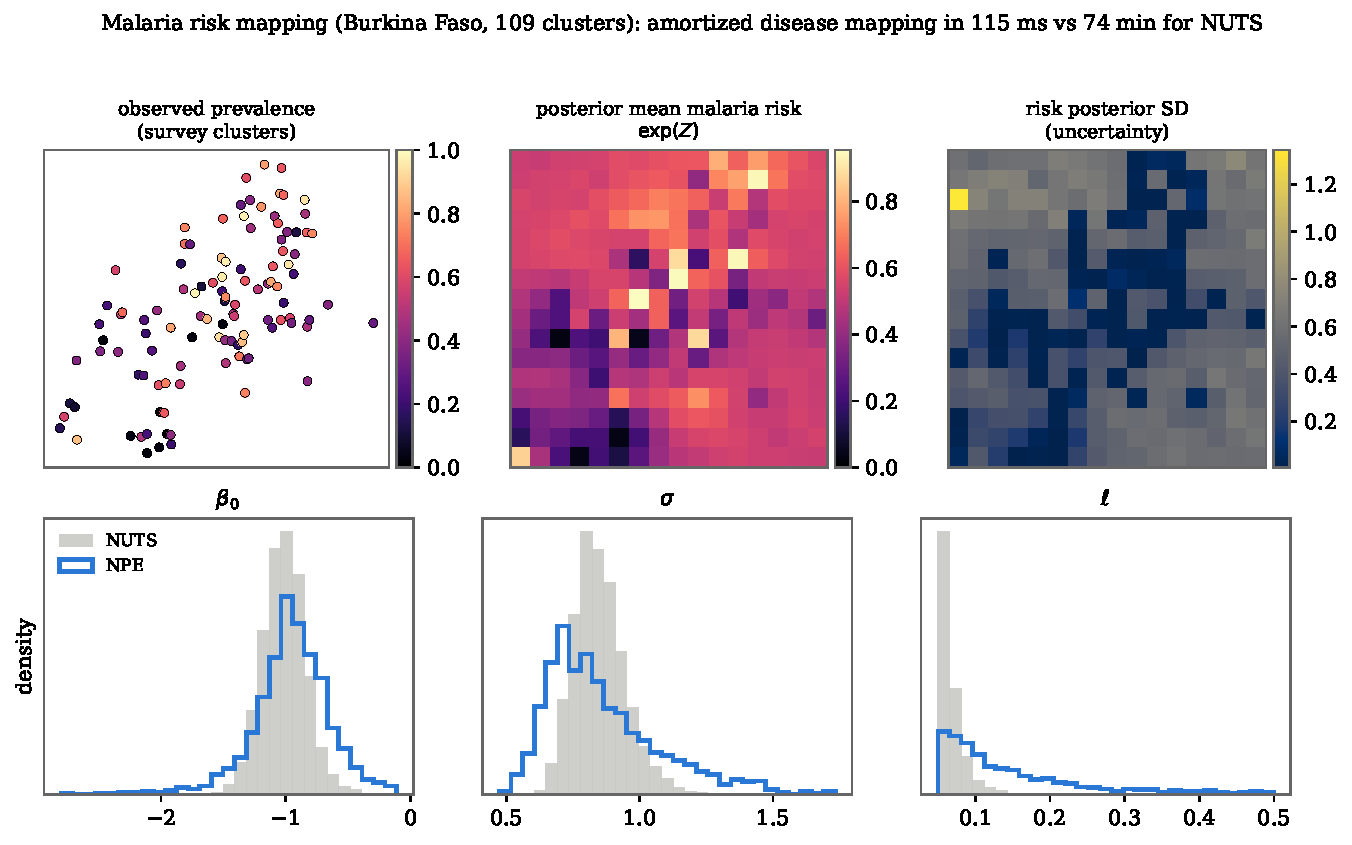
\includegraphics[width=\textwidth]{figures/fig_malaria.pdf}
\caption{Malaria risk mapping from Burkina Faso parasite-rate surveys.
\emph{Top:} observed cluster prevalence; the posterior mean risk surface
$\exp(Z)$; and its uncertainty. \emph{Bottom:} amortized parameter posteriors
(blue) versus gold-standard NUTS (grey) for the Poisson-offset LGCP.}
\label{fig:malaria}
\end{figure}

\section{Related work}

\paragraph{Simulation-based inference.}
NPE originates with mixture-density and flow-based conditional estimators
\citep{papamakarios2016fast}, refined by sequential and automatic-posterior
variants \citep{lueckmann2017flexible,greenberg2019automatic} and surveyed by
\citet{cranmer2020frontier}. Alternatives estimate the likelihood
\citep{papamakarios2019sequential} or the likelihood ratio
\citep{hermans2020likelihood}; \citet{lueckmann2021benchmarking} benchmark them.
Our density estimator is a masked autoregressive flow
\citep{papamakarios2017masked,rezende2015variational}. Calibration is assessed
with simulation-based calibration \citep{talts2018validating} and the classifier
two-sample test \citep{lopez2017revisiting}; recent work stresses that SBI must be
checked, not assumed \citep{hermans2022trust}.

\paragraph{Inference for LGCPs and spatial models.}
Classical LGCP inference uses MCMC over the latent field
\citep{moller1998log,christensen2005robust}, with elliptical slice sampling and
manifold methods to cope with the field--hyperparameter coupling
\citep{murray2010elliptical,girolami2011riemann}. INLA with an SPDE
representation \citep{rue2009approximate,lindgren2011explicit,simpson2016going}
is the dominant fast, approximate alternative. These are all \emph{per-dataset}
solvers; our contribution is orthogonal---an amortized posterior shared across
datasets---and complementary, since INLA or NUTS can serve as the gold standard
we validate against.

\paragraph{Neural inference for spatial and point-process models.}
Amortized and likelihood-free neural inference has moved rapidly into spatial
statistics and ecology; see \citet{zammitmangion2025neural} for a review. Two
threads are directly relevant. The first estimates parameters as \emph{point
predictions}: \citet{vihrs2022using} trains neural networks to recover
spatial point-process parameters from a pattern, and neural Bayes estimators
provide fast, amortized point estimators for spatial covariance and extremal
models, with bootstrap uncertainty
\citep{gerber2021fast,lenzi2023neural,sainsbury2024likelihood,sainsbury2023neural}.
Our regressor baseline is a representative of this thread, and our calibration
analysis quantifies precisely what its uncertainty does and does not deliver. The
second thread learns \emph{full posteriors}: closest to us,
\citet{wang2025inference} apply BayesFlow \citep{radev2020bayesflow} to one- and
two-dimensional LGCPs and validate against MCMC on selected realizations, with an
oral-microbiome application. We are complementary to that work: rather than a new
application, we contribute a systematic \emph{trustworthiness audit}---calibration
across the entire prior via SBC, a controlled comparison against the
point-estimate paradigm, a summary-statistic ablation, a classifier-two-sample
and Wasserstein benchmark against MCMC in two dimensions, and a
kernel-misspecification stress
test---using a deliberately minimal, from-scratch estimator so that the
conclusions are about the approach, not a particular software stack.

\section{Discussion}

We have shown that amortized NPE gives calibrated posteriors for LGCP parameters
that match gold-standard MCMC at a fraction of the per-dataset cost, and that the
common regression shortcut, while accurate in the mean, is dangerously
overconfident. The recipe is simple and dependency-light: simulate, embed with a
CNN, fit a flow, and---critically---\emph{check} with SBC, coverage and a
gold-standard comparison before trusting the result.

\paragraph{Limitations and outlook.}
Our study fixes the grid resolution and the kernel family; the misspecification
analysis shows real sensitivity to smoothness, and the field posterior, though
calibrated, uses a low-rank Gaussian form that may understate strongly
non-Gaussian tails. Two directions we have begun here seem the most consequential.
The intensity-surface posterior (Section~\ref{sec:field}) turns amortized
inference into amortized \emph{mapping}, the object practitioners act on; richer
posterior families (conditional flows or diffusions over the field) and joint
inference with the hyperparameters are natural refinements. The
preferential-sampling and change-of-support results
(Sections~\ref{sec:pref}--\ref{sec:agg}) show that once amortized inference is
\emph{trusted}, the likelihood-free interface makes non-standard observation
models tractable almost for free; thinning and imperfect detection, and adaptive
designs are immediate further members of that family. The most important gap is
external validity---all our experiments are simulated; a real application, where
the generative model is itself uncertain, is the essential next step. Amortizing
over grid resolution and domain shape, and
treating the kernel smoothness as an inferred parameter to convert the
misspecification sensitivity into robustness, round out the agenda. We view
calibrated amortized inference---of parameters, surfaces, and observation
processes alike---as a practical path to LGCP modelling at the scale and
observational complexity that contemporary spatial data demand.

\paragraph{Reproducibility.}
The simulator, method, diagnostics and all experiment scripts are released; every
figure and number in this paper is regenerated by the accompanying code.

\small
\bibliographystyle{plainnat}
\bibliography{refs}

\end{document}
